%=========================
% Sections/03-CongTrinhLienQuan.tex
% Chương 3 – Các công trình liên quan
%=========================
\section{Công nghệ liên quan}
\subsection{Các mô hình kiến trúc phần mềm}

Kiến trúc hệ thống là một trong những yếu tố quan trọng quyết định khả năng mở rộng, hiệu năng và tính linh hoạt của hệ thống phần mềm. Kiến trúc phần mềm mô tả cấu trúc tổng thể của hệ thống, bao gồm các thành phần chính, mối quan hệ giữa các thành phần và cách chúng tương tác với nhau trong quá trình xử lý dữ liệu.

Trong các hệ thống hiện đại, đặc biệt là hệ thống trí tuệ nhân tạo trong lĩnh vực thương mại điện tử, kiến trúc hệ thống cần hỗ trợ xử lý phân tán, tích hợp nhiều dịch vụ AI và đảm bảo khả năng mở rộng linh hoạt theo tải hệ thống. Các mô hình kiến trúc phổ biến hiện nay bao gồm monolithic architecture, microservice architecture và cloud-native architecture.

%=========================
\subsubsection{Monolithic Architecture}

Monolithic architecture là mô hình kiến trúc trong đó toàn bộ hệ thống được xây dựng và triển khai như một khối thống nhất. Các thành phần như giao diện người dùng, logic nghiệp vụ và tầng truy cập dữ liệu thường nằm trong cùng một ứng dụng, chia sẻ chung mã nguồn, môi trường chạy và quy trình triển khai.

Như trình bày ở \Cref{fig:monolithic_architecture}, toàn bộ hệ thống được triển khai trong một khối thống nhất.

\begin{figure}[H]
    \centering
    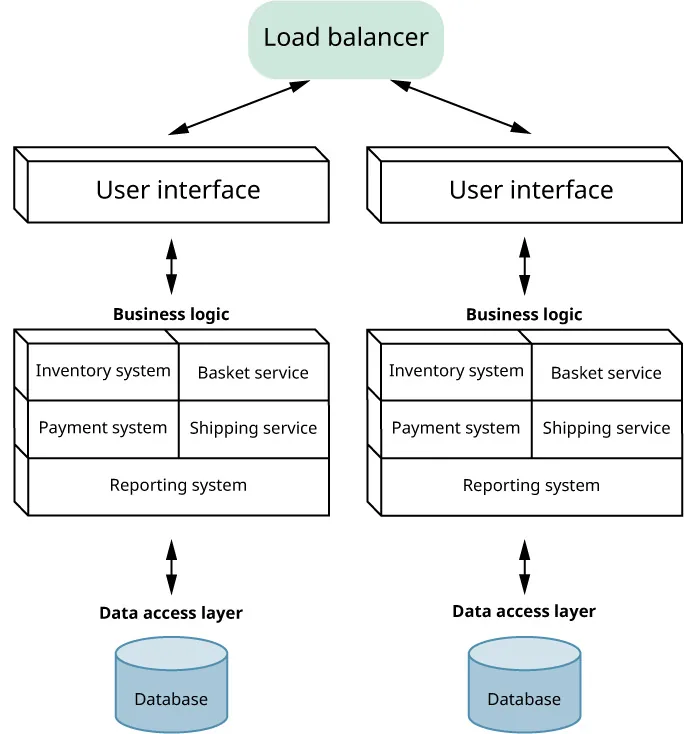
\includegraphics[width=0.5\textwidth]{Images/Congnghelienquan/Monolithic_architecture.png}
    \caption[Kiến trúc monolithic trong đó toàn bộ thành phần hệ thống được triển khai trong một ứng dụng duy nhất (nguồn: OpenStax)]{Kiến trúc monolithic trong đó toàn bộ thành phần hệ thống được triển khai trong một ứng dụng duy nhất (nguồn: OpenStax \parencite{openstax_cloud_native_intro})}
    \label{fig:monolithic_architecture}
\end{figure}

Trong kiến trúc monolithic, toàn bộ hệ thống thường nằm trong một codebase duy nhất, các module chia sẻ chung tài nguyên và giao tiếp nội bộ trong cùng tiến trình. Cách tổ chức này giúp việc phát triển, kiểm thử và triển khai ban đầu trở nên đơn giản, đặc biệt phù hợp với các hệ thống nhỏ hoặc các phiên bản thử nghiệm ban đầu.

Ưu điểm của monolithic architecture là cấu trúc dễ hiểu, ít phức tạp trong triển khai và có hiệu năng tốt do không phát sinh overhead mạng giữa các thành phần. Tuy nhiên, khi hệ thống phát triển lớn hơn, kiến trúc này có thể gặp khó khăn trong việc mở rộng, bảo trì và cập nhật từng chức năng riêng lẻ. Sự phụ thuộc chặt giữa các module cũng khiến việc thay đổi một thành phần có thể ảnh hưởng đến toàn bộ hệ thống.

%=========================
\subsubsection{Microservice Architecture}

Microservice architecture là mô hình kiến trúc trong đó hệ thống được chia thành nhiều dịch vụ nhỏ, độc lập và giao tiếp với nhau thông qua API. Mỗi service thường đảm nhiệm một chức năng nghiệp vụ riêng, có thể được phát triển, kiểm thử, triển khai và mở rộng độc lập với các service khác.

Như trình bày ở \Cref{fig:microservice_architecture}, hệ thống được phân tách thành các service độc lập.

\begin{figure}[H]
    \centering
    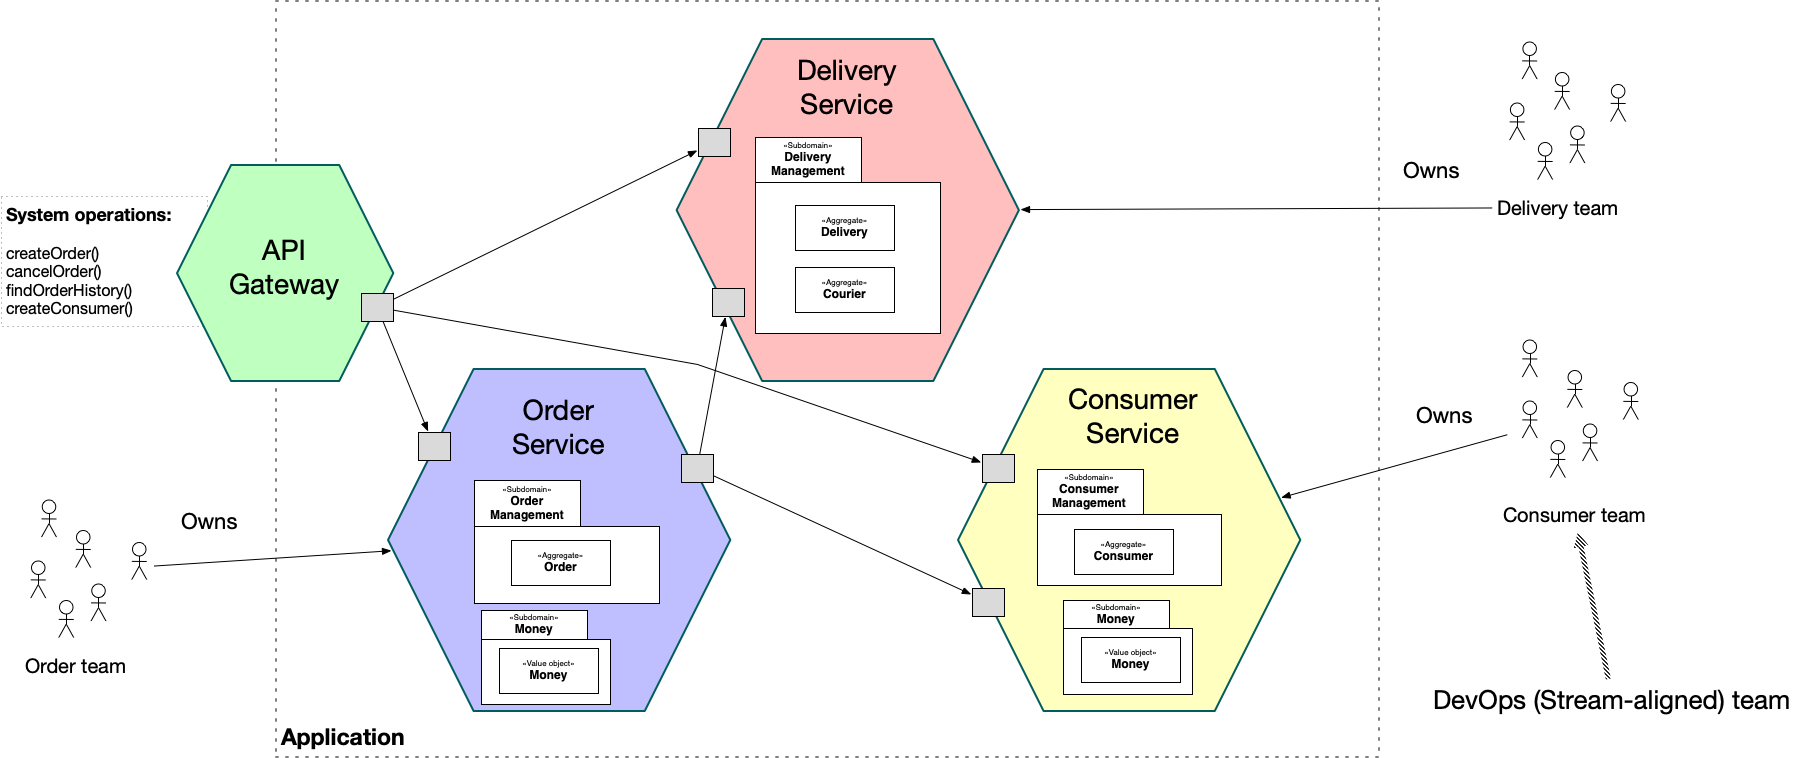
\includegraphics[width=0.85\textwidth]{Images/Congnghelienquan/microservices-teams-subdomains.png}
    \caption[Kiến trúc microservice trong đó hệ thống được chia thành các dịch vụ nhỏ, độc lập và giao tiếp qua API (nguồn: Microservices.io)]{Kiến trúc microservice trong đó hệ thống được chia thành các dịch vụ nhỏ, độc lập và giao tiếp qua API (nguồn: Microservices.io \parencite{microservices_io_patterns})}
    \label{fig:microservice_architecture}
\end{figure}

Trong kiến trúc microservice, hệ thống được tổ chức thành nhiều service độc lập, mỗi service phụ trách một nhóm chức năng cụ thể và giao tiếp với nhau thông qua REST API, gRPC hoặc message broker. Các service có thể được phát triển bằng công nghệ khác nhau tùy theo yêu cầu nghiệp vụ, miễn là chúng tuân thủ cơ chế giao tiếp đã được thiết kế.

Ưu điểm của microservice architecture là khả năng mở rộng linh hoạt theo từng thành phần, hỗ trợ phát triển song song giữa các nhóm và tăng khả năng chịu lỗi của hệ thống. Khi một service gặp sự cố, các service khác vẫn có thể tiếp tục hoạt động nếu hệ thống được thiết kế tốt.

Tuy nhiên, microservice cũng làm tăng độ phức tạp trong vận hành vì hệ thống trở thành một môi trường phân tán. Việc triển khai, monitoring, logging, tracing và orchestration cần được quản lý chặt chẽ. Ngoài ra, giao tiếp giữa các service có thể phát sinh overhead mạng và làm tăng độ trễ so với kiến trúc monolithic.
%=========================
\subsubsection{Service-based Architecture}

Service-based architecture là mô hình kiến trúc trong đó hệ thống được chia thành nhiều service độc lập theo từng nhóm chức năng hoặc nghiệp vụ. Mỗi service đảm nhiệm một vai trò cụ thể và giao tiếp với các service khác thông qua API. Cách tiếp cận này giúp hệ thống dễ mở rộng, dễ bảo trì và phù hợp với các hệ thống có nhiều thành phần xử lý riêng biệt như tìm kiếm, gợi ý sản phẩm, quản lý người dùng và xử lý AI.

Khác với monolithic architecture, service-based architecture không gom toàn bộ chức năng vào một ứng dụng duy nhất. Thay vào đó, hệ thống được tổ chức thành các service có trách nhiệm rõ ràng. Tuy nhiên, mô hình này không nhất thiết phải tách nhỏ đến mức microservices hoàn chỉnh, mà có thể chia theo các module lớn hơn để giảm độ phức tạp trong triển khai.

Như trình bày ở \Cref{fig:service_based_architecture}, hệ thống service-based được tổ chức thành nhiều service độc lập và giao tiếp với nhau thông qua API.

\begin{figure}[H]
    \centering
    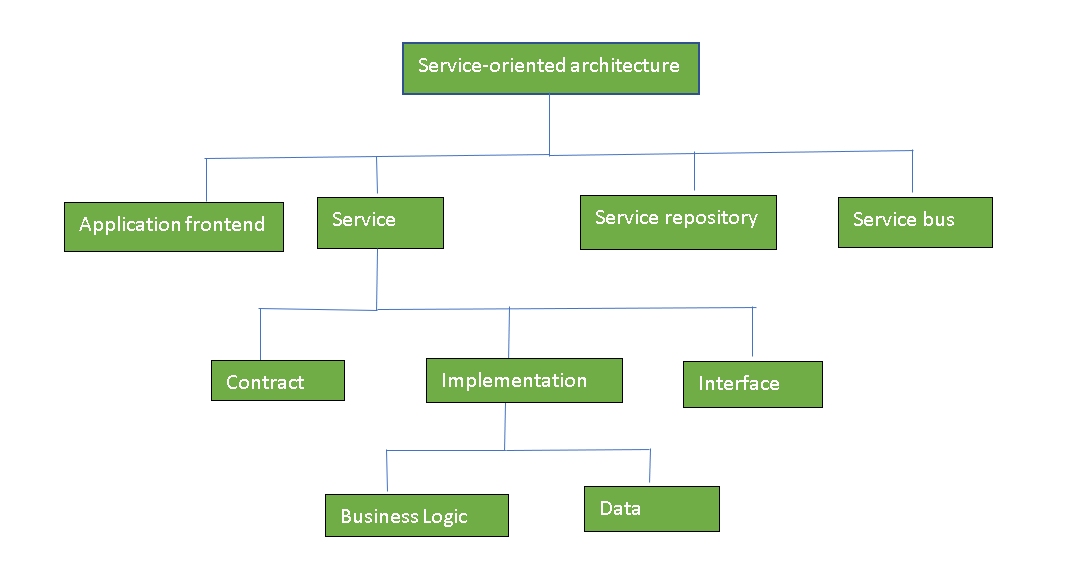
\includegraphics[width=0.85\textwidth]{Images/Congnghelienquan/service-base-architectural.png}
    \caption[Kiến trúc service-based chia hệ thống thành nhiều service độc lập và giao tiếp thông qua API]{Kiến trúc service-based chia hệ thống thành nhiều service độc lập và giao tiếp thông qua API \parencite{geeksforgeeks2023soa}}
    \label{fig:service_based_architecture}
\end{figure}

Trong service-based architecture, hệ thống được chia thành các service theo chức năng, mỗi service có thể được phát triển, bảo trì và mở rộng tương đối độc lập. Các service giao tiếp với nhau thông qua API, giúp giảm sự phụ thuộc trực tiếp giữa các module so với monolithic architecture.

Ưu điểm của kiến trúc này là dễ mở rộng từng thành phần, dễ thay đổi hoặc nâng cấp một service mà không ảnh hưởng quá nhiều đến toàn bộ hệ thống. Mô hình này cũng phù hợp với các hệ thống có nhiều thành phần riêng biệt như search service, recommendation service, user service, LLM service và vector database service.

Tuy nhiên, service-based architecture yêu cầu thiết kế API rõ ràng giữa các service. Việc quản lý giao tiếp, đồng bộ dữ liệu và xử lý lỗi giữa các service cũng phức tạp hơn so với monolithic architecture. Ngoài ra, hệ thống có thể phát sinh độ trễ khi các service gọi nhau thông qua mạng.

%=========================
\subsubsection{So sánh kiến trúc hệ thống}

Như tổng hợp ở Bảng \Cref{tab:architecture_comparison}, các kiến trúc được so sánh dựa trên khả năng mở rộng, mức độ triển khai, bảo trì và sự phù hợp với hệ thống AI.

\begin{table}[H]
\centering
\caption{So sánh các kiến trúc hệ thống phổ biến trong ứng dụng AI hiện đại}
\label{tab:architecture_comparison}
\renewcommand{\arraystretch}{1.3}

\begin{tabularx}{\linewidth}{|>{\raggedright\arraybackslash}X|>{\raggedright\arraybackslash}X|>{\raggedright\arraybackslash}X|>{\raggedright\arraybackslash}X|}
\hline
\textbf{Tiêu chí} & \textbf{Monolithic} & \textbf{Microservice} & \textbf{Service-based} \\ \hline
Khả năng mở rộng & Thấp & Cao & Rất cao \\ \hline
Triển khai & Đơn giản & Trung bình & Phức tạp \\ \hline
Bảo trì & Khó & Dễ & Dễ hơn monolithic \\ \hline
Hiệu năng & Tốt (nhỏ) & Ổn định & Tối ưu cho các service lớn \\ \hline
Phù hợp AI system & Thấp & Cao & Rất cao \\ \hline
\end{tabularx}
\end{table}

Tổng kết lại, kiến trúc microservice và service-based là lựa chọn phù hợp cho các hệ thống AI hiện đại nhờ khả năng mở rộng linh hoạt, hỗ trợ triển khai phân tán và tích hợp tốt với các thành phần như vector database, embedding models và các dịch vụ AI.
%=========================
\subsection{Backend Framework}
\subsubsection{ASP.NET Core (.NET)}

ASP.NET Core là framework xây dựng ứng dụng web và API trong hệ sinh thái .NET, sử dụng ngôn ngữ C\# và hỗ trợ triển khai đa nền tảng \parencite{ch4_aspnet_overview}. Framework cung cấp middleware, dependency injection, xác thực và phân quyền để tổ chức xử lý yêu cầu và nghiệp vụ.

Trong Wispace, ASP.NET Core được lựa chọn để xây dựng các dịch vụ Core, Learning \& Exam, Assessment và Progress \& Reporting. AIHub sử dụng backend ASP.NET Core riêng theo modular monolith, phục vụ quản lý tổ chức, khóa API, hạn mức và các công cụ học thuật nội bộ. Các tác vụ suy luận được tách sang dịch vụ Python FastAPI.

\textbf{Ứng dụng trong hệ thống:}
\begin{itemize}
    \item Xây dựng API cho luyện tập, thi thử, kết quả và quản trị Wispace.
    \item Quản lý tổ chức, quyền truy cập API và usage của AIHub.
    \item Truy cập PostgreSQL qua EF Core và Npgsql; schema được quản lý riêng bằng Flyway và SQL migration.
    \item Điều phối công việc nền qua RabbitMQ và gọi dịch vụ AI bằng HTTP.
\end{itemize}

%=========================

\subsubsection{FastAPI}

FastAPI là framework Python dùng để xây dựng API theo chuẩn ASGI, hỗ trợ lập trình bất đồng bộ, kiểm tra dữ liệu dựa trên khai báo kiểu và tự động sinh tài liệu OpenAPI \parencite{fastapidocs2024}. Framework phù hợp để cung cấp giao diện gọi mô hình AI và tích hợp các thư viện xử lý tiếng nói, học máy trong Python.

Trong Wispace, FastAPI cung cấp API cho pipeline chấm Speaking gồm M5 xử lý âm học, M6 đánh giá ngôn ngữ và M7 tổng hợp kết quả. Đối với AIHub, FastAPI cung cấp giao diện thực thi dịch vụ mô hình và sinh nội dung học thuật. Backend ASP.NET Core quản lý nghiệp vụ, quyền truy cập và hạn mức trước khi gọi dịch vụ AI.

\textbf{Ứng dụng trong hệ thống:}
\begin{itemize}
    \item Tiếp nhận audio và ngữ cảnh câu hỏi để thực thi pipeline chấm Speaking.
    \item Kiểm tra dữ liệu đầu vào, trả điểm và nhận xét theo hợp đồng API thống nhất.
    \item Cung cấp API cho các tác vụ AI của AIHub, tách xử lý mô hình khỏi backend nghiệp vụ.
\end{itemize}

%=========================

\subsubsection{Node.js}

Node.js là môi trường runtime JavaScript được xây dựng trên V8 engine của Google Chrome nhằm hỗ trợ phát triển ứng dụng phía server \parencite{nodejsdocs2024}. Node.js sử dụng mô hình event-driven và non-blocking I/O giúp tối ưu khả năng xử lý đồng thời và giảm chi phí tài nguyên trong các hệ thống có lượng request lớn.

Khác với các kiến trúc xử lý đồng bộ truyền thống, Node.js cho phép hệ thống xử lý nhiều kết nối đồng thời thông qua cơ chế asynchronous programming. Điều này giúp Node.js phù hợp với các ứng dụng realtime hoặc các dịch vụ cần phản hồi nhanh.

Trong các hệ thống backend hiện đại, Node.js thường được sử dụng cho các thành phần realtime hoặc lightweight service.

%=========================
\subsubsection{So sánh Backend Framework}

Nhằm làm rõ sự khác biệt giữa các backend framework, Bảng \Cref{tab:backend_framework} tổng hợp so sánh dựa trên các tiêu chí quan trọng như hiệu năng, khả năng hỗ trợ AI và mức độ phù hợp với hệ thống phân tán.

\begin{table}[H]
\centering
\caption{So sánh các backend framework phổ biến dựa trên hiệu năng, khả năng hỗ trợ AI và mức độ phù hợp với kiến trúc hệ thống phân tán}
\label{tab:backend_framework}
\renewcommand{\arraystretch}{1.3}

\begin{tabularx}{\linewidth}{|>{\raggedright\arraybackslash}X|>{\raggedright\arraybackslash}X|>{\raggedright\arraybackslash}X|>{\raggedright\arraybackslash}X|}
\hline
\textbf{Tiêu chí} & \textbf{ASP.NET Core} & \textbf{FastAPI} & \textbf{Node.js} \\ \hline
Ngôn ngữ & C\# & Python & JavaScript \\ \hline
Hiệu năng & Cao & Rất cao & Cao \\ \hline
Hỗ trợ AI/ML & Trung bình & Rất tốt & Thấp \\ \hline
Microservices & Rất tốt & Tốt & Tốt \\ \hline
Realtime & Tốt & Trung bình & Rất tốt \\ \hline
Ứng dụng phù hợp & Enterprise backend & AI services & Realtime systems \\ \hline
\end{tabularx}
\end{table}

Wispace và AIHub kết hợp ASP.NET Core cho API, nghiệp vụ và truy cập dữ liệu với Python FastAPI cho các dịch vụ AI. Node.js được khảo sát như một lựa chọn phát triển backend, không phải thành phần backend được lựa chọn trong thiết kế này. Việc tách lớp nghiệp vụ khỏi suy luận cho phép triển khai và điều chỉnh tài nguyên theo đặc điểm từng nhóm xử lý.

\subsection{Frontend Framework}

Frontend framework đóng vai trò quan trọng trong việc xây dựng UI , đảm bảo UX , khả năng tương tác và hiệu năng hiển thị của hệ thống. Trong các hệ thống hiện đại như AI Shopping Assistant, frontend không chỉ đảm nhiệm việc hiển thị dữ liệu mà còn hỗ trợ tìm kiếm thông minh, cập nhật realtime và tương tác đa phương tiện với backend và AI services.

%=========================
\subsubsection{React}

React là một thư viện JavaScript do Meta phát triển, được thiết kế theo kiến trúc component-based \textcite{reactdocs2024}. React sử dụng Virtual DOM nhằm tối ưu hiệu năng khi cập nhật giao diện người dùng.

React được sử dụng để xây dựng hai frontend độc lập cho Wispace Speaking và AIHub, quản lý giao diện và tương tác người dùng thông qua API của backend tương ứng.

Như trình bày ở các ứng dụng web hiện đại, React đặc biệt phù hợp với các hệ thống có dữ liệu động và yêu cầu cập nhật giao diện theo thời gian thực.

\textbf{Ứng dụng trong hệ thống:}
\begin{itemize}
    \item Wispace: xây dựng giao diện kho đề, luyện tập, ghi âm và thi thử IELTS Speaking.
    \item Hiển thị trạng thái chấm, điểm, nhận xét và lịch sử tiến bộ; cung cấp giao diện quản trị và kiểm duyệt nội dung Wispace.
    \item AIHub: xây dựng Portal quản lý tổ chức, khóa API, dịch vụ và lịch sử sử dụng.
    \item Cung cấp giao diện Academic Lab để sinh mẫu, hiệu đính, thẩm định và xuất dữ liệu học thuật.
\end{itemize}

React có ưu điểm về tính linh hoạt cao, hệ sinh thái lớn và khả năng mở rộng tốt cho các ứng dụng web hiện đại.

%=========================
\subsubsection{Angular}

Angular là framework frontend toàn diện do Google phát triển, dựa trên TypeScript \textcite{angulardocs2024}. Framework này cung cấp sẵn các thành phần như routing, form handling, dependency injection và state management.

Angular thường được sử dụng trong các hệ thống doanh nghiệp có độ phức tạp cao và yêu cầu kiến trúc chặt chẽ.

\textbf{Ứng dụng trong thực tế:}
\begin{itemize}
    \item Ứng dụng doanh nghiệp lớn (enterprise applications)
    \item Hệ thống dashboard và admin panel phức tạp
    \item Các hệ thống yêu cầu kiến trúc chuẩn hóa cao
\end{itemize}

Angular có ưu điểm về kiến trúc rõ ràng và tính nhất quán cao, tuy nhiên độ phức tạp lớn hơn so với React.

%=========================
\subsubsection{Vue}

Vue.js là framework frontend nhẹ, linh hoạt và dễ tiếp cận \textcite{vuedocs2024}. Vue kết hợp ưu điểm của React  và Angular , nhưng đơn giản hơn trong quá trình triển khai.

Vue thường được sử dụng trong các dự án có yêu cầu phát triển nhanh hoặc quy mô nhỏ đến trung bình.

\textbf{Ứng dụng trong thực tế:}
\begin{itemize}
    \item Website thương mại điện tử nhỏ và vừa
    \item Prototype hoặc MVP development
    \item Ứng dụng cần phát triển nhanh
\end{itemize}

Vue phù hợp với nhóm phát triển nhỏ nhờ cú pháp đơn giản và khả năng học nhanh.

%=========================
\subsubsection{So sánh frontend framework}

Nhằm làm rõ sự khác biệt giữa các frontend framework, Bảng \Cref{tab:frontend_framework_comparison} tổng hợp so sánh dựa trên các tiêu chí như hiệu năng, độ phức tạp và mức độ phù hợp với hệ thống AI.

\begin{table}[H]
\centering
\caption{So sánh các frontend framework phổ biến dựa trên kiến trúc, hiệu năng và mức độ phù hợp với hệ thống AI hiện đại}
\label{tab:frontend_framework_comparison}
\renewcommand{\arraystretch}{1.3}

\begin{tabularx}{\linewidth}{|>{\raggedright\arraybackslash}X|>{\raggedright\arraybackslash}X|>{\raggedright\arraybackslash}X|>{\raggedright\arraybackslash}X|}
\hline
\textbf{Tiêu chí} & \textbf{React} & \textbf{Angular} & \textbf{Vue} \\ \hline
Loại & Library & Full framework & Progressive framework \\ \hline
Ngôn ngữ & JavaScript/JSX & TypeScript & JavaScript \\ \hline
Hiệu năng & Cao & Cao & Cao \\ \hline
Độ phức tạp & Trung bình & Cao & Thấp \\ \hline
Hệ sinh thái & Rất lớn & Lớn & Trung bình \\ \hline
Độ linh hoạt & Rất cao & Trung bình & Cao \\ \hline
Phù hợp AI system & Rất tốt & Tốt & Trung bình \\ \hline
\end{tabularx}
\end{table}

Trong hệ thống AI Shopping Assistant, React được lựa chọn làm frontend chính nhờ khả năng linh hoạt cao, hỗ trợ tốt cho giao diện động và khả năng tích hợp dễ dàng với các API AI cũng như dữ liệu realtime từ backend services.
\subsection{Công nghệ xử lý tiếng nói}

Xử lý tiếng nói cung cấp transcript và các đặc trưng phục vụ đánh giá Speaking. Các công đoạn gồm nhận dạng nội dung, phát hiện vùng có tiếng nói, căn chỉnh thời gian từ và tổng hợp tiếng nói để phát câu hỏi.

\subsubsection{Nhận dạng tiếng nói tự động}

Nhận dạng tiếng nói tự động (Automatic Speech Recognition -- ASR) chuyển audio thành văn bản. Whisper được xây dựng theo hướng học từ dữ liệu tiếng nói có giám sát yếu ở quy mô lớn \parencite{ch3_whisper}. Trong pipeline Wispace, Whisper large-v3 được chọn làm cấu hình cơ sở để cung cấp transcript cho phân tích ngôn ngữ và đặc trưng thời gian. Qwen3-ASR là một phương án khảo sát khác, cung cấp các mô hình nhận dạng đa ngôn ngữ \parencite{ch3_qwen_asr}.

Việc so sánh ASR cần xét chất lượng transcript, khả năng bảo toàn lỗi và sự ngập ngừng của người nói, độ trễ và tài nguyên sử dụng trên cùng tập audio. Transcript trôi chảy không đồng nghĩa với nhận dạng nguyên lời: thao tác tự sửa ngữ pháp hoặc bỏ từ lặp có thể làm sai bằng chứng chấm ngôn ngữ. Vì vậy, hệ thống lưu nguồn ASR và metadata chất lượng cùng transcript, thay vì coi mọi đầu ra là bản chép đã xác minh.

\subsubsection{Phát hiện hoạt động giọng nói}

Voice Activity Detection (VAD) xác định các khoảng có tiếng nói trong audio. Silero VAD cung cấp mô hình tiền huấn luyện để phát hiện các khoảng này \parencite{ch3_silero}. So với cách chỉ xét mức năng lượng, VAD dựa trên mô hình học có thể khai thác các đặc trưng phức tạp hơn; chất lượng vẫn phụ thuộc điều kiện thu âm và cần kiểm tra trên dữ liệu sử dụng thực tế.

Wispace sử dụng VAD để xác định lượng tiếng nói có thể xử lý và phát hiện bài ghi âm không đủ điều kiện. Ngưỡng đầu vào được cấu hình theo Part vì độ dài câu trả lời khác nhau. VAD không xác định nội dung đúng hay sai và không tự tạo điểm phát âm. Các khoảng thời gian trong audio gốc cần được bảo toàn để phục vụ phân tích khoảng dừng.

\subsubsection{Căn chỉnh thời gian từ}

Forced alignment xác định vị trí thời gian của transcript trên audio, khác với ASR là nhận dạng nội dung. WhisperX kết hợp nhận dạng, VAD và căn chỉnh để cung cấp mốc thời gian ở mức từ. Các mốc này hỗ trợ tính tốc độ nói, khoảng dừng và liên kết nhận xét với đoạn audio tương ứng.

Wispace dùng WhisperX cho bước căn chỉnh sau ASR. Transcript và mốc thời gian phải cùng nguồn; từ không căn chỉnh được được giữ trạng thái thiếu dữ liệu, không gán thời gian giả định. Điểm tin cậy của aligner phản ánh phép căn chỉnh, không được hiểu thành xác suất transcript đúng hoặc điểm IELTS đáng tin cậy.

\begin{figure}[H]
    \centering
    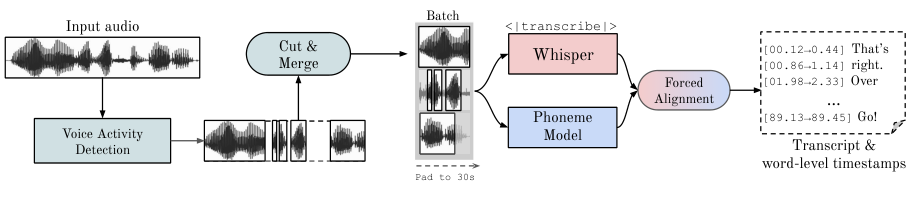
\includegraphics[width=\linewidth]{Images/Congnghelienquan/whisperx_pipeline.png}
    \caption[Pipeline nhận dạng và căn chỉnh thời gian từ của WhisperX]{Pipeline nhận dạng và căn chỉnh thời gian từ của WhisperX \parencite{ch3_whisperx}}
    \label{tech:fig:whisperx-pipeline}
\end{figure}

\subsubsection{Tổng hợp tiếng nói}

Text-to-Speech (TTS) chuyển văn bản thành tiếng nói. Các mô hình như VITS tiếp cận bài toán tổng hợp đầu cuối, kết hợp mô hình sinh và học đối kháng \parencite{ch3_vits}. Khi lựa chọn giải pháp tự triển khai hoặc dịch vụ TTS, cần cân nhắc độ rõ của giọng đọc, độ trễ, chi phí và khả năng lưu lại audio đã sinh.

Trong Wispace, TTS phục vụ phát câu hỏi và hướng dẫn trong luyện tập hoặc thi thử. Audio câu hỏi được chuẩn bị hoặc cache theo phiên bản nội dung và cấu hình giọng, giúp chuyển câu không phụ thuộc việc sinh tiếng nói tại thời điểm thi. TTS không tham gia đánh giá chất lượng câu trả lời của học viên.

\subsection{Các phương pháp đánh giá IELTS Speaking tự động}

IELTS Speaking sử dụng bốn tiêu chí: Fluency and Coherence, Lexical Resource, Grammatical Range and Accuracy và Pronunciation \parencite{ch3_ielts_scoring}. Hệ thống tự động cần kết hợp bằng chứng âm học và ngôn ngữ; một chỉ số như tốc độ nói hoặc độ chính xác transcript không thể đại diện đầy đủ cho cả bốn tiêu chí.

\subsubsection{Đánh giá phát âm}

Các phương pháp đánh giá phát âm có thể khai thác sự phù hợp giữa âm thanh và đơn vị ngôn ngữ, hoặc học quan hệ giữa biểu diễn âm thanh với điểm người chấm. HuBERT học biểu diễn tiếng nói thông qua dự đoán đơn vị ẩn; wav2vec 2.0 là một hướng học tự giám sát khác cho biểu diễn tiếng nói \parencite{ch3_wav2vec2}. Các encoder này cần được kết hợp với bộ dự đoán và dữ liệu nhãn phù hợp để phục vụ chấm điểm.

\begin{figure}[H]
    \centering
    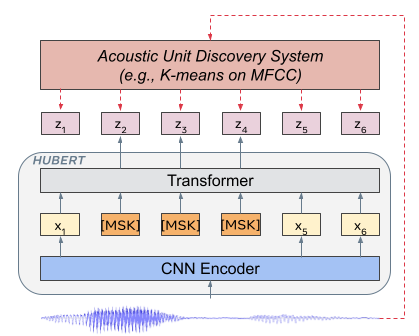
\includegraphics[width=.72\linewidth]{Images/Congnghelienquan/hubert_architecture.png}
    \caption[Cơ chế tiền huấn luyện HuBERT]{Cơ chế tiền huấn luyện HuBERT bằng dự đoán đơn vị ẩn tại các vị trí bị che \parencite{ch3_hubert}}
    \label{tech:fig:hubert-pretraining}
\end{figure}

Hình \ref{tech:fig:hubert-pretraining} minh họa cơ chế tiền huấn luyện HuBERT. Trong pipeline chấm Speaking, Wispace sử dụng HuBERT-base đóng băng tầng 9, tổng hợp đặc trưng, chuẩn hóa, giảm chiều bằng PCA và dự đoán bằng LightGBM cho nhánh Pronunciation của M5. Cách tiếp cận này giữ encoder cố định và huấn luyện bộ dự đoán phía sau. Điểm tổng từ biểu diễn audio không tự chứng minh khả năng xác định chính xác lỗi từng âm; phản hồi chi tiết cần có bằng chứng và phương pháp đánh giá tương ứng.

\subsubsection{Đánh giá độ trôi chảy}

Độ trôi chảy có thể được mô tả bằng tốc độ nói, tốc độ phát âm, độ dài chuỗi nói giữa các khoảng dừng và phân bố khoảng dừng. Cách tính cần thống nhất đơn vị, khoảng thời gian được xét và quy tắc loại trừ đoạn không có tiếng nói. Các dấu hiệu lặp hoặc tự sửa cũng có thể hỗ trợ phân tích, nhưng chịu ảnh hưởng của việc ASR giữ hay bỏ các hiện tượng này.

Nhánh M5 của Wispace kết hợp đặc trưng thời gian bằng luật cấu hình theo Part, cho phép giải thích đóng góp của từng chỉ số. Luật ban đầu cần được kiểm tra và hiệu chỉnh bằng dữ liệu người chấm. Fluency âm học không bao gồm toàn bộ Coherence; tốc độ nhanh hoặc ít khoảng dừng không đương nhiên tương ứng với điểm cao.

\subsubsection{Đánh giá ngôn ngữ}

Nhánh ngôn ngữ phân tích transcript trong ngữ cảnh câu hỏi để đánh giá phạm vi và cách dùng từ vựng, cấu trúc ngữ pháp và tổ chức ý. Các hướng tiếp cận gồm đặc trưng ngôn ngữ kết hợp mô hình dự đoán, mô hình ngôn ngữ được huấn luyện cho tác vụ và đánh giá theo rubric với đầu ra có cấu trúc. Việc lựa chọn cần xét khả năng dẫn chứng, tính ổn định và mức phù hợp với điểm người chấm.

M6 được thiết kế để đánh giá Lexical Resource, Grammatical Range and Accuracy và cung cấp bằng chứng Coherence. Nhận xét gắn với đoạn transcript và ngữ cảnh câu hỏi; metadata ASR giúp nhận biết vùng dữ liệu chưa chắc chắn. Một lỗi do ASR tạo ra không được mặc định quy thành lỗi của học viên, cũng không xem câu đã được ASR sửa là bằng chứng sử dụng ngôn ngữ chính xác.

\subsubsection{Tổng hợp và hiệu chuẩn điểm}

Tổng hợp kết quả kết hợp các nguồn bằng chứng; hiệu chuẩn điều chỉnh quan hệ giữa đầu ra mô hình với thang đánh giá mục tiêu. Hai bước này cần được phân biệt với việc chỉ làm tròn số. Dữ liệu hiệu chuẩn và đánh giá phải được tách phù hợp, đặc biệt theo người nói, để hạn chế kết quả quá lạc quan do cùng học viên xuất hiện ở nhiều tập.

M7 được thiết kế để tổng hợp đầu ra M5 và M6, hình thành bốn điểm tiêu chí, band tổng và phản hồi thống nhất. Fluency âm học được kết hợp với bằng chứng Coherence thay vì coi hai đại lượng là một. Công thức tổng hợp, quy tắc làm tròn và phiên bản hiệu chuẩn được quản lý rõ ràng. Đánh giá sử dụng sai số, tương quan và mức nhất quán với người chấm; không mặc định lấy trung bình điểm từng câu để xác định band toàn bài thi.

\subsection{Công nghệ lưu trữ và xử lý bất đồng bộ}

Hai hệ thống cần lưu dữ liệu nghiệp vụ, quản lý tệp và xử lý các tác vụ có thời gian thực thi khác nhau. Cơ sở dữ liệu, kho đối tượng, hàng đợi và cache đảm nhiệm các vai trò riêng, không thay thế lẫn nhau.

\subsubsection{Cơ sở dữ liệu quan hệ}

PostgreSQL và MySQL với InnoDB đều hỗ trợ giao dịch và các ràng buộc quan hệ, phù hợp với dữ liệu tài khoản, quyền truy cập và lịch sử xử lý \parencite{ch4_postgresql_transactions,ch3_mysql_innodb}. Việc lựa chọn cần dựa trên mô hình dữ liệu, thư viện tích hợp và yêu cầu vận hành, thay vì xếp hạng hiệu năng chung cho mọi loại truy vấn.

PostgreSQL được chọn cho Wispace và AIHub nhờ phù hợp với mô hình dữ liệu quan hệ và khả năng tích hợp .NET qua Npgsql. Dữ liệu nghiệp vụ có cấu trúc được lưu bằng bảng, khóa và ràng buộc; JSON có thể dùng cho một số đầu ra mô hình linh hoạt. Các dịch vụ Wispace sở hữu dữ liệu riêng, AIHub có database độc lập. Schema được quản lý bằng SQL migration của Flyway, còn EF Core đảm nhiệm ánh xạ và truy cập dữ liệu.

\subsubsection{Lưu trữ đối tượng}

Lưu trữ đối tượng tổ chức tệp theo khóa định danh, phù hợp với audio và tệp xuất có kích thước lớn. S3 hỗ trợ cấp quyền tải lên hoặc tải xuống có thời hạn qua presigned URL \parencite{ch3_s3_presigned}. So với lưu nội dung tệp trực tiếp trong bảng nghiệp vụ, cách tổ chức này cho phép tách đường truyền tệp và chính sách lưu trữ khỏi truy vấn quan hệ.

Wispace lưu audio trên S3; PostgreSQL giữ object key, kích thước, checksum và trạng thái xác minh. AIHub sử dụng kho đối tượng cho tệp xuất dữ liệu học thuật. Backend kiểm tra quyền trước khi cấp URL; URL tạm không thay thế bước kiểm tra tệp và xác nhận bài nộp.

\subsubsection{Hàng đợi thông điệp}

Hàng đợi giúp tách thời điểm tiếp nhận yêu cầu khỏi thời điểm xử lý. RabbitMQ hỗ trợ publisher confirm và consumer acknowledgement cho các giai đoạn giao nhận thông điệp \parencite{ch4_rabbitmq_confirms}; prefetch giới hạn số thông điệp chưa xác nhận được giao cho consumer. Kafka tổ chức sự kiện theo topic và partition, hỗ trợ retention và đọc lại bằng offset \parencite{ch4_kafka_intro}.

\begin{table}[H]
\centering
\caption{Đối chiếu RabbitMQ và Kafka theo nhu cầu của đề tài}
\label{tech:tab:broker-comparison}
\small
\renewcommand{\arraystretch}{1.2}
\begin{tabularx}{\linewidth}{|>{\raggedright\arraybackslash}X|>{\raggedright\arraybackslash}X|>{\raggedright\arraybackslash}X|}
\hline
\textbf{Tiêu chí} & \textbf{RabbitMQ trong thiết kế} & \textbf{Kafka khi áp dụng} \\ \hline
Phân phối công việc & Queue cho nhóm worker, xác nhận từng thông điệp. & Cần phối hợp trạng thái job với cách tiêu thụ topic và quản lý offset. \\ \hline
Khai thác lịch sử & Queue phục vụ vận chuyển; dữ liệu gốc do database quản lý. & Retention và offset hỗ trợ nhiều nhóm đọc lại luồng sự kiện. \\ \hline
Công việc kéo dài & Kết hợp prefetch và giới hạn đồng thời của worker. & Cần thiết kế tiến độ xử lý, phân vùng và phân công lại consumer phù hợp. \\ \hline
Nhu cầu đề tài & Chấm Speaking, tác vụ AI dài và xuất dữ liệu nền. & Cân nhắc khi cần nền tảng phân tích luồng hoặc đọc lại lượng lớn sự kiện. \\ \hline
\end{tabularx}
\end{table}

RabbitMQ được chọn vì thiết kế ưu tiên điều phối công việc chấm và tác vụ nền. Lựa chọn này không khẳng định RabbitMQ luôn nhanh hơn hoặc Kafka không thể xử lý tác vụ. Thông điệp chỉ chứa định danh và tham chiếu; audio nằm trong S3. Trạng thái job, outbox và cơ chế chống trùng được lưu bền vững để hỗ trợ xử lý lại; broker không tự bảo đảm một tác vụ chỉ chạy đúng một lần.

\subsubsection{Bộ nhớ đệm}

Redis cung cấp các cấu trúc dữ liệu trong bộ nhớ để lưu dữ liệu cần truy cập nhanh \parencite{ch4_redis}. Cache giúp giảm truy vấn lặp đối với nội dung và cấu hình ít thay đổi; thời hạn và cơ chế cập nhật cache cần phù hợp với nguồn dữ liệu. Redis cũng có thể hỗ trợ bộ đếm giới hạn tốc độ truy cập.

Wispace dùng Redis cho nội dung đề và cấu hình thường đọc; AIHub dùng cho cấu hình dịch vụ và giới hạn tốc độ theo tổ chức hoặc khóa API. Điểm số, bài nộp và sổ hạn mức có thẩm quyền vẫn do PostgreSQL quản lý. Rate limit kiểm soát tần suất gửi yêu cầu, còn quota là quyền sử dụng nghiệp vụ; hai cơ chế cần được phân biệt.

\subsection{Công nghệ cung cấp và quản lý dịch vụ AI}

Cung cấp AI qua API cần kết hợp thực thi mô hình với quản lý hợp đồng dữ liệu, phiên bản, quyền truy cập và lịch sử sử dụng. Đây là cơ sở cho đường gọi nội bộ của Wispace và dịch vụ B2B của AIHub.

\subsubsection{Cung cấp mô hình qua API}

OpenAPI mô tả đường dẫn, dữ liệu yêu cầu, phản hồi và cơ chế bảo mật của HTTP API \parencite{ch3_openapi}. Hợp đồng rõ ràng giúp backend nghiệp vụ và dịch vụ Python phát triển độc lập, đồng thời hỗ trợ kiểm thử tương thích khi thay đổi cấu trúc dữ liệu.

Tác vụ ngắn có thể trả kết quả đồng bộ; tác vụ dài trả mã công việc để bên gọi theo dõi trạng thái. Wispace Assessment gọi lớp điều phối chấm Speaking bằng FastAPI, nơi M5, M6 và M7 được phối hợp theo hợp đồng đánh giá. AIHub kiểm tra yêu cầu B2B trước khi chuyển đến dịch vụ mô hình. Cả hai cần trạng thái lỗi rõ ràng và mã chống trùng cho các thao tác có thể được gửi lại.

\subsubsection{Quản lý phiên bản và định tuyến mô hình}

Một phiên bản mô hình gồm không chỉ trọng số mà còn cấu hình tiền xử lý, tokenizer, schema đầu ra và các quy tắc hậu xử lý liên quan. Thay đổi một thành phần có thể làm kết quả khác nhau; vì vậy mỗi phản hồi cần truy vết được cấu hình thực thi tương ứng.

Wispace gắn kết quả với phiên bản pipeline và hiệu chuẩn. AIHub sử dụng model route để ánh xạ dịch vụ với mô hình hoặc nhà cung cấp được cấu hình. Phương án dự phòng chỉ được dùng khi tương thích với chức năng và hợp đồng dữ liệu; mô hình sinh nội dung không mặc định thay thế Scoring Model. Khi thay phiên bản, cần kiểm tra dữ liệu, chất lượng và khả năng tương thích trước khi chuyển lưu lượng.

\subsubsection{Quản lý truy cập và sử dụng API}

Quản lý API kết hợp xác thực bên gọi, phân quyền dịch vụ, giới hạn tốc độ và kiểm soát hạn mức. Khóa API nhận diện một ứng dụng hoặc đối tác, nhưng quyền truy cập vẫn cần được kiểm tra theo tổ chức, dịch vụ và trạng thái credentials. Bí mật được sử dụng từ máy chủ đối tác, không đưa vào frontend công khai.

AIHub quản lý tổ chức B2B, khóa API, gói dịch vụ và usage. Wispace quản lý quyền học viên và hạn mức luyện tập hoặc thi thử tại lớp nghiệp vụ riêng. Với tác vụ dài, hạn mức được giữ, chốt hoặc giải phóng theo trạng thái xử lý; yêu cầu gửi lại phải được nhận diện để tránh tính lặp. Usage ghi định danh yêu cầu, phiên bản mô hình, thời gian xử lý và đơn vị tiêu thụ phục vụ theo dõi, đối soát.

\subsubsection{Quản lý dữ liệu học thuật}

Dữ liệu học thuật cần lưu nguồn, phiên bản và quyết định thẩm định, tách đầu ra AI ban đầu khỏi bản chỉnh sửa. Dữ liệu SFT gồm đầu vào và đầu ra mục tiêu; dữ liệu DPO gồm các phương án được chọn và bị từ chối cho cùng đầu vào. DPO tối ưu theo dữ liệu ưu tiên tương đối thay vì chỉ học một đầu ra mục tiêu \parencite{ch3_dpo}.

Academic Lab của AIHub tổ chức quá trình sinh mẫu, hiệu đính, thẩm định và xuất bộ dữ liệu có phiên bản. Chỉ mẫu đáp ứng điều kiện mới được đưa vào bản xuất; cần kiểm tra quyền sử dụng, thông tin cá nhân và trùng lặp giữa các tập. Dữ liệu Writing SFT/DPO phục vụ tác vụ tương ứng, không mặc định trở thành nhãn chấm Speaking. Với Wispace, dữ liệu audio và điểm người chấm được quản lý theo sự đồng ý của học viên và mục đích huấn luyện, hiệu chuẩn, đánh giá.
